% !TEX program = xelatex

\documentclass{beamer}
\usepackage[utf8]{inputenc}
\usepackage{listings}
\usepackage{fontspec} % 定制字体
\usepackage{xeCJK}
\usepackage{utopia} %font utopia imported
%\usepackage[UTF8,noindent]{ctexcap}
\usepackage{latexsym,amssymb,amsmath,amsbsy,amsopn,amstext,xcolor,multicol}
\usepackage{graphicx,wrapfig,fancybox}
\usepackage{booktabs}
% \usetheme{Rochester}
\usetheme{Madrid}
\usecolortheme{default}
 % 衬线字体:Linux Libertine
    % BoldFont 可以选择 Bold 字重或者 Semibold 字重
    % BoldItalicFont 也有对应 BoldFont 的字重选择
    % 这里使用 Semibold 字重
  %   \setmainfont{LinLibertine_R.otf}[
  %     BoldFont = LinLibertine_RZ.otf,
  %     ItalicFont = LinLibertine_RI.otf,
  %     BoldItalicFont = LinLibertine_RZI.otf]
  % % % 无衬线字体:Linux Biolinum
  % \setsansfont{LinBiolinum_R.otf}[
  %     BoldFont = LinBiolinum_RB.otf,
  %     ItalicFont = LinBiolinum_RI.otf,
  %     BoldItalicFont = LinBiolinum_RBO.otf]
  % % 等宽/打印机字体:Linux Libertine Mono
  % \setmonofont{LinLibertine_M.otf}[
  %     BoldFont = LinLibertine_MB.otf,
  %     ItalicFont = LinLibertine_MO.otf,
  %     BoldItalicFont  = LinLibertine_MBO.otf]
  % \setCJKmainfont[ItalicFont={AR PL UKai CN},
  % BoldFont={WenQuanYi Micro Hei}]{IPAMinCho,IPA明朝}
  \setCJKsansfont{WenQuanYi Micro Hei}
  \setCJKmonofont{WenQuanYi Micro Hei Mono}

  \newfontfamily\menlo{WenQuanYi Micro Hei Mono}
  \usepackage{xcolor} % 定制颜色
  \definecolor{mygreen}{rgb}{0,0.6,0}
  \definecolor{mygray}{rgb}{0.5,0.5,0.5}
  \definecolor{mymauve}{rgb}{0.58,0,0.82}
  \lstset{ %
  backgroundcolor=\color{white},      % choose the background color
  basicstyle=\footnotesize\ttfamily,  % size of fonts used for the code
  columns=fullflexible,
  tabsize=4,
  breaklines=true,               % automatic line breaking only at whitespace
  captionpos=b,                  % sets the caption-position to bottom
  commentstyle=\color{mygreen},  % comment style
  escapeinside={\%*}{*)},        % if you want to add LaTeX within your code
  keywordstyle=\color{blue},     % keyword style
  stringstyle=\color{mymauve}\ttfamily,  % string literal style
  frame=single,
  rulesepcolor=\color{red!20!green!20!blue!20},
  % identifierstyle=\color{red},
  language=c++,
  }
%------------------------------------------------------------
%This block of code defines the information to appear in the
%Title page
\title[毕设开题] %optional
{基于域名解析数据的DNS劫持分析}

% \subtitle{波长检测型表面等离子体共振 (SPR) 传感}

\author[芦迪] % (optional)
{芦迪 }

\institute[THU, EE] % (optional)
{
  指导老师:李星 \\
  \
  
  Department of Electronic Engineering,\\
  Tsinghua University
  
}

\date[2018.1.12] % (optional)
{January 12, 2018}

\logo{
\includegraphics[height=1.5cm]{images/thuee-logo.png}}

%End of title page configuration block
%------------------------------------------------------------



%------------------------------------------------------------
%The next block of commands puts the table of contents at the 
%beginning of each section and highlights the current section:

\AtBeginSection[]
{
  \begin{frame}
    \frametitle{目录}
    \tableofcontents[currentsection]
  \end{frame}
}
%------------------------------------------------------------


\begin{document}
%The next statement creates the title page.
\frame{\titlepage}


%---------------------------------------------------------
%This block of code is for the table of contents after
%the title page
\begin{frame}
\frametitle{目录}
\tableofcontents
\end{frame}
%---------------------------------------------------------


\section{背景介绍}

%---------------------------------------------------------
%Changing visivility of the text
\begin{frame}{DNS介绍}
  DNS:Domain Name System
  \begin{itemize}
    \item 一个分层的分布式命名系统,将域名转换为IP地址
    \item 指定每个域的权威域名服务器分配域名,层层分配
  \end{itemize}
  \begin{figure}
  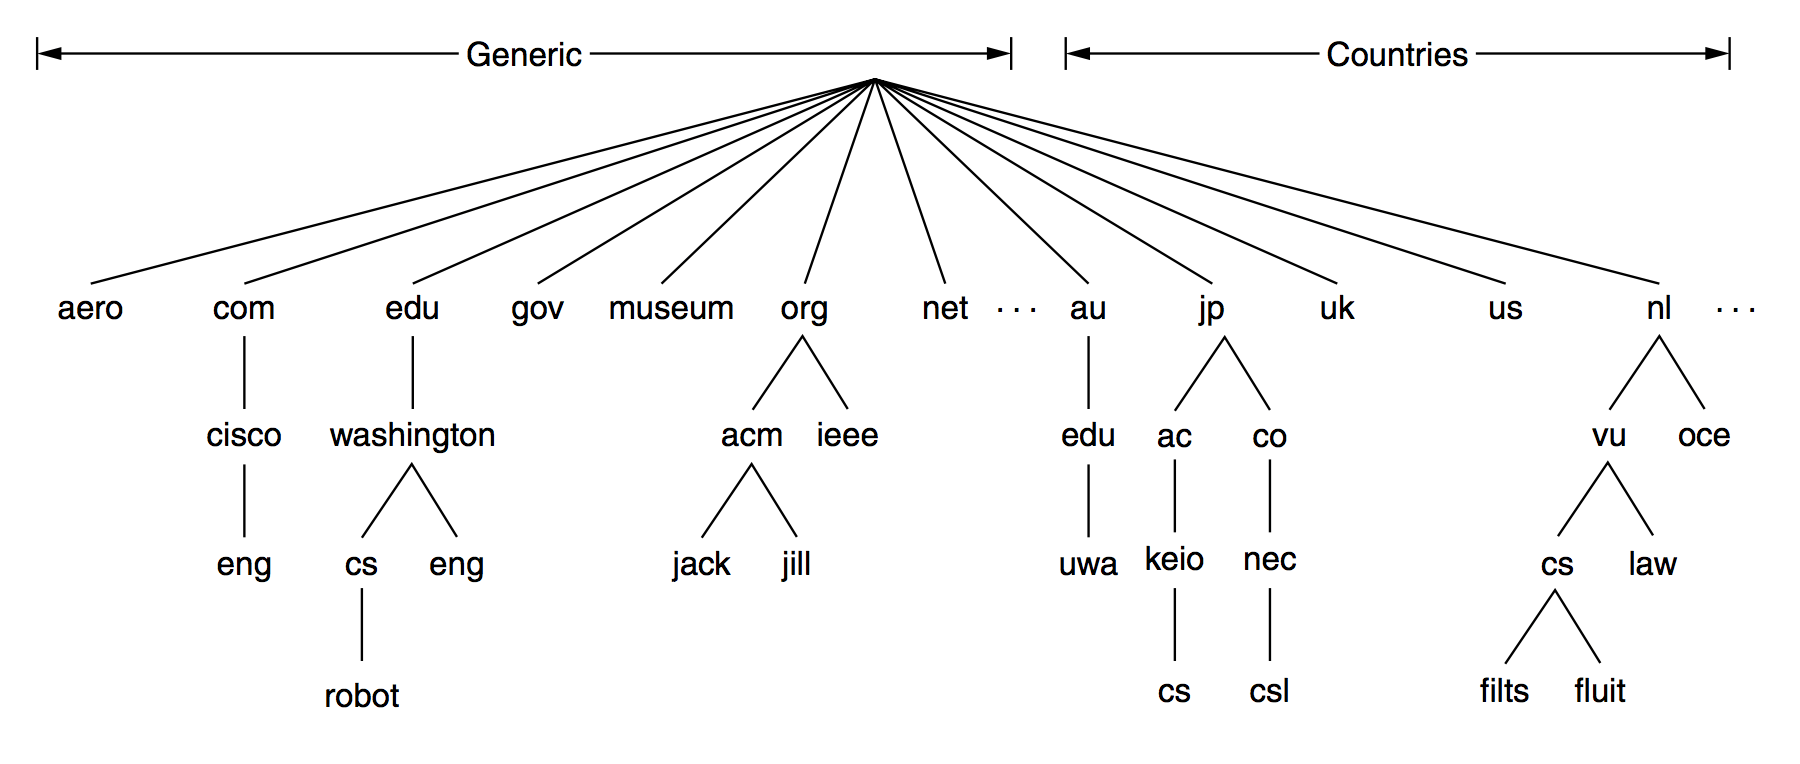
\includegraphics[height=3cm,width=7.07cm]{images/domain_tree.png}
  \caption{Domain Tree}
  \end{figure}
  DNSSEC:公钥密码机制,添加数字签名,协议增强

\end{frame}

\begin{frame}{DNS介绍}
  域名解析过程:
  \begin{figure}
  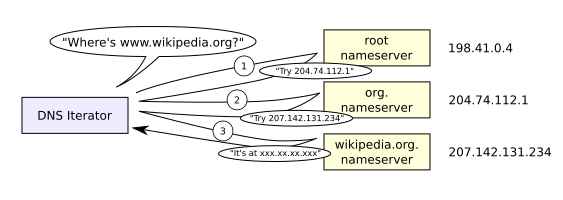
\includegraphics[height=3cm,width=8.455cm]{images/Example_of_an_iterative_DNS_resolver.png}
  \end{figure}
  % \pause

  常见记录类型:
  \begin{table}
    \scriptsize
  \begin{tabular}{r|l}
    \toprule
    记录类型& 含义\\
    \midrule
    A& 主机的IPv4地址\\
    AAAA& 主机的IPv6地址\\
    NS& 该域名所在域的权威域名服务器\\
    CNAME& 将当前域名映射到另一个域名\\
    MX & 将域名映射到该域的邮件传输代理列表 \\
    PTR&反向DNS查找指针\\
    \bottomrule
    \end{tabular}
  \end{table}
\end{frame}

\begin{frame}{CDN与负载均衡}
  CDN:Content Delivery Network
  \begin{itemize}
    \item 部署边缘服务器,使用户就近获取所需内容,降低网络拥塞
    \item 依靠CNAME记录,实现网络请求重定向
  \end{itemize}
  \begin{figure}
  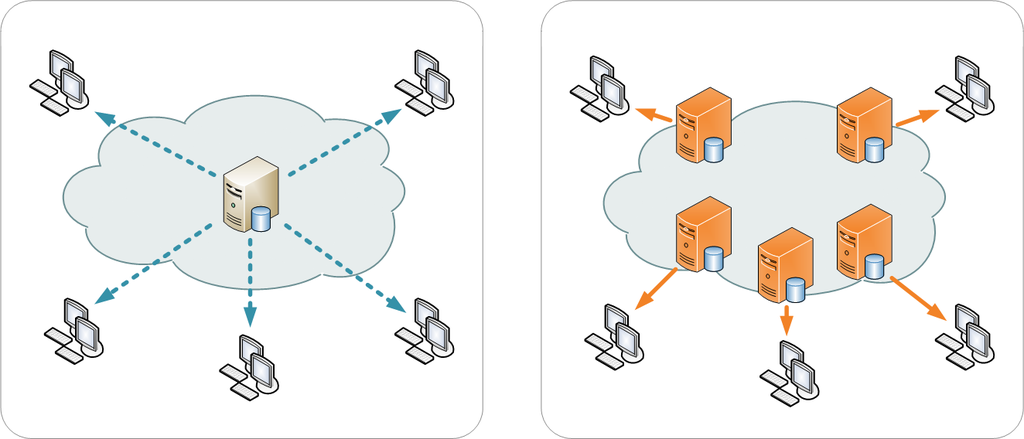
\includegraphics[height=3cm,width=7.07cm]{images/NCDNCDN.png}
  \end{figure}

  负载均衡
  \begin{itemize}
    \item DNS轮循是负载均衡的一种方法
  \end{itemize}
\end{frame}

\section{毕设内容}




\frame{\frametitle{DNS 请求格式}
\begin{columns}
\begin{column}{0.5\textwidth}
  \begin{figure}
    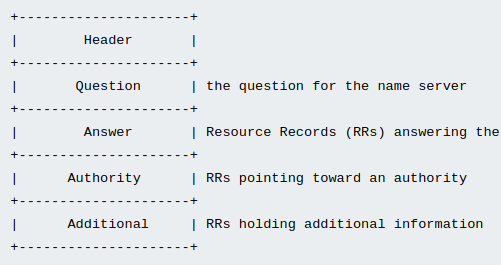
\includegraphics[height=2.65cm,width=5cm]{images/dnsmessage.png}
    \caption{DNS Message}
    \end{figure}
\end{column}
\begin{column}{0.5\textwidth}

  \begin{figure}
    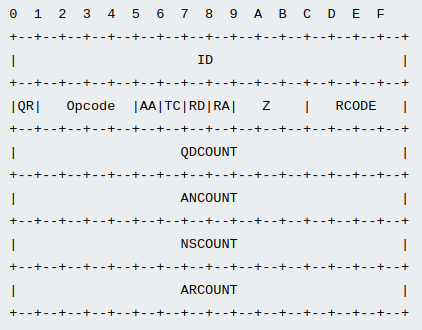
\includegraphics[height=3.9cm,width=5cm]{images/dnsheader.png}
    \caption{DNS Header}
    \end{figure}
\end{column}
\end{columns}
}

\begin{frame}{资源记录分析}
  我们希望通过分析解析数据,了解目前IPv6与DNSSEC普及情况:
  \begin{enumerate}
    \item 根据A记录与AAAA记录,判断IPv6支持情况
    \begin{figure}
      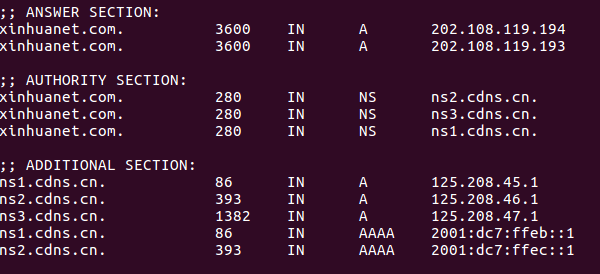
\includegraphics[height=2.74cm,width=6cm]{images/aaaa.png}
    \end{figure} 

    \item 根据RRSIG记录,判断DNSSEC支持情况
    \begin{figure}
      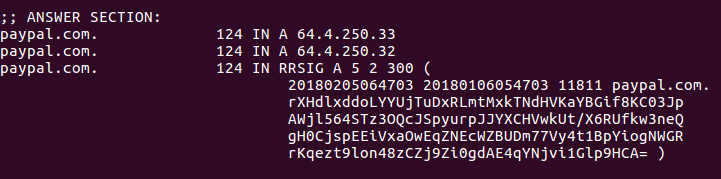
\includegraphics[height=1.79cm,width=7.21cm]{images/dnssec.png}
    \end{figure} 
  \end{enumerate}

\end{frame}

\begin{frame}{DNS解析返回类型分析}

  \begin{itemize}
    \item 通过DNS解析,由域名得到IP地址,存在以下类别:
  \begin{enumerate}
    \item 返回唯一IP
    \item CDN
    \item 负载均衡
    \item DNS劫持
    \item 缓存中毒或其他有害情况
  \end{enumerate}
  \item 我们的目的是实现一个系统,对DNS解析的结果进行分类
  \end{itemize}
  
\end{frame}

\section{操作方法}

\begin{frame}{数据获取}
  \begin{columns}
    \begin{column}{0.5\textwidth}
      \small{收集 Open Resolvers 数据及Domain Names 数据,进行DNS解析测试}
      
      \begin{table}
        \scriptsize
      \begin{tabular}{l|l}
        \toprule
        Open Resolvers& Top Domain Names\\
        \midrule
        114.114.114.114 & baidu.com \\
        8.8.8.8 & qq.com \\
        4.2.2.2&     taobao.com \\
        9.9.9.9&  sina.com.cn \\
        
        8.26.56.26& youku.com \\
        
        199.91.73.222& soso.com \\
        
        156.154.71.1& sohu.com \\
        
        199.85.126.10& 163.com \\
        ......&...... \\
        \bottomrule
        \end{tabular}
      \end{table}
    \end{column}
    \begin{column}{0.5\textwidth}
    
      \begin{figure}
        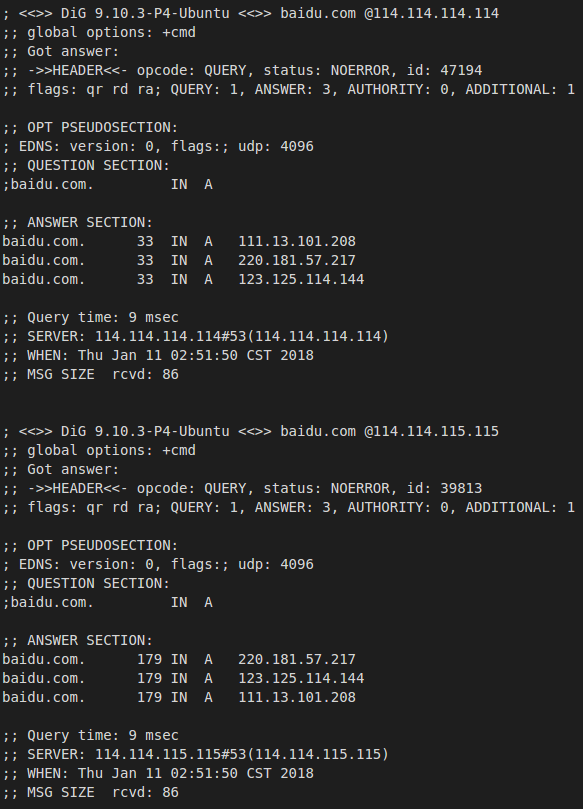
\includegraphics[height=8.09cm,width=5.83cm]{images/digres.png}
        \caption{DNS Header}
        \end{figure}
    \end{column}
    \end{columns}
  
\end{frame}

\begin{frame}{数据分析}

  \begin{itemize}
    \item CDN 解析的结果通常包含有CNAME记录
    \item 关于DNS劫持的检测,文献\cite{Yan2006}提出了一种基于贝叶斯原理的判别方法
  \end{itemize}

\end{frame}

\section{未来工作计划}

\begin{frame}{未来工作计划}

  \begin{itemize}
    \item 继续文献调研,研究对负载均衡、缓存中毒等类别DNS解析结果的判别方法
    \item 进一步收集Open Resolvers,获取数据进行分析
  \end{itemize}

\end{frame}


 \begin{frame}{参考文献}
  \scriptsize
  \bibliographystyle{unsrt}%Used BibTeX style is unsrt
  \bibliography{ref.bib}
\end{frame}

\begin{frame}
  \begin{figure}
    
\includegraphics[height=2.23cm,width=4.29cm]{images/thank.jpg}
  \end{figure} 
\end{frame}
\end{document}

%---------------------------------------------------------


%---------------------------------------------------------
%Example of the \pause command
% \begin{frame}
%   \frametitle{实验原理}
% In this slide \pause

% the text will be partially visible \pause

% And finally everything will be there
% \end{frame}
%---------------------------------------------------------

% \section{实验原理}

% %---------------------------------------------------------
% %Highlighting text
% \begin{frame}{检测原理}
% % \frametitle
% \begin{itemize}
%   \item 表面等离子体共振(简称SPR)是一种物理光学现象,利用光在玻璃界面处发生全内反射时的消逝波,激发出沿金属薄膜表面传播的表面等离子体波(SPW)
%   \item 在入射角或波长为某一适当值的条件下,入射光与 SPW 发生共振,此时全反射的反射光能量急剧下降,在反射光谱上出现共振吸收峰
% \end{itemize}
% \begin{figure}
%   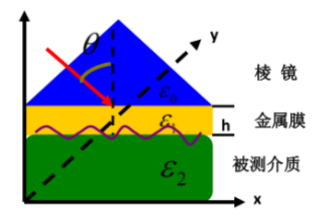
\includegraphics[height=2.86cm,width=4.29cm]{images/2_2.png}
%   \caption{棱镜型 SPR 传感器结构}
% \end{figure}
% \end{frame}
% \begin{frame}{检测原理}
%   \begin{itemize}
%     \item 当紧靠在金属薄膜表面的介质折射率不同时, 共振峰位置将不同
%     \item SPR 的共振峰位置与被测介质的性质密切相关, 根据对这个信号的检测就可以获得被测物质的折射率、浓度、膜层厚度、反应进程等信息, 从而达到生化检测的目的
%   \end{itemize}
%   \begin{figure}
%     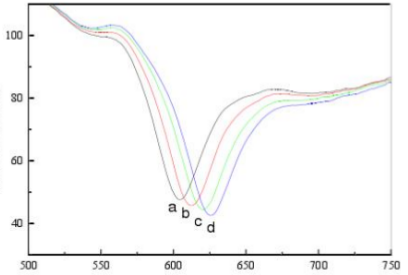
\includegraphics[height=3.575cm,width=5.304cm]{images/2_1.png}
%     \caption{波长调制检测方法对不同物质检测的仿真结果}
%   \end{figure}
% \end{frame}

% %---------------------------------------------------------
% % 
% %---------------------------------------------------------

% \section{理论仿真}
% \begin{frame}{理论仿真}
%   利用MATLAB软件对波长检测型SPR传感结果进行仿真,并研究了实验条件对检测结果的影响,用以对实验条件建设提供理论依据。结论如下:
%   \begin{enumerate}
%     \item 当被测物质一定时,入射角变小,共振波长变大,共振半峰宽度变大,共振深度增大灵敏度变大。
%     \item 当入射角度不变时,被测物质折射率增大,共振波长变大,共振半峰宽度变大,共振深度增大,灵敏度变大。
%     \item 存在一个合适大小的金属膜厚度使得实验效果最好,反射率最低点最低吸收效果最好而且半峰宽较窄。本次仿真中的最佳结果为 50nm,当厚度小于 50 时半峰宽较大而且吸收峰的共振深度较小;当厚度大于 50nm 时半峰宽降低但是吸收峰共振深度也减小。
%     \item 入射角度的改变会使得被测物质的检测范围发生改变。入射角度变大,检测范围变大,检测灵敏度变小。
%   \end{enumerate}
  
% \end{frame}

% \section{实验系统}
% \begin{frame}{实验系统}
%   \begin{itemize}
%     \item 实验所用SPR检测系统依据Kretchsmann棱镜型结构和波长调制原理搭建,主体结构如下:
%     \begin{figure}
%       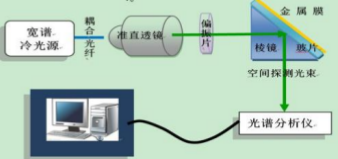
\includegraphics[height=3.29cm,width=7cm]{images/2_3.png}
%     \end{figure}
%   \end{itemize}
  

% \begin{block}{装置简述}
%   \begin{description}
%     \item[入射光路] 宽谱光源 + 光纤 + 准直镜 + 偏振片,产生宽谱平行光
%     \item[传感探头] Kretchsmann棱镜型结构,采用金膜作为金属膜
%     \item[信号采集] 聚焦棱镜 + 多模光纤 + SMA接头 + 光纤光谱仪
%   \end{description}
% \end{block}
  
% \end{frame}
% \begin{frame}
%   \frametitle{实验系统}
%   \begin{figure}
%     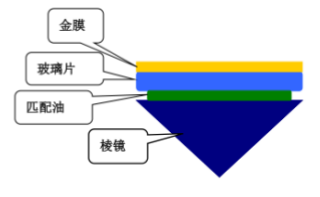
\includegraphics[height=3.94cm,width=6.4cm]{images/2_4.png}
%     \caption{探头的结构}
%   \end{figure}
% \end{frame}

% \section{方法步骤}
% \begin{frame}{光路调整}
%   \begin{enumerate}
%     \item 入射角调到需要的角度,根据发射机上的角度刻度值实现
%     \item 调节棱镜和发射机的高度使得传感区位于棱镜底部的中心位置,使用擦镜纸在棱镜两侧相同距离处观察光斑的垂直位置,基本保证两个光斑在同一竖直高度即可
%     \item 打开电脑光谱仪,接收棱镜反射回来的光,调整接收机使得收到的光谱尽量的大。这一步是实验中最困难的,要确保光线与接收机同轴。接收机接收处可以发现两个光斑,分别为棱镜和接收机后光纤端面反射过来的,应调整接收机角度、高度,使得这两个光斑尽量重合与接收面中心处
%   \end{enumerate}
% \end{frame}
% \begin{frame}{系统实验}
%   \begin{enumerate}
%     \item 设定棱镜全反射光作为参考光,用于波长域上归一化处理
%     \item 放置金膜:注意清洁,先滴匹配油,再用镊子将金片放置在棱镜上,注意将金属膜朝上放置
%     \item 将光谱仪软件调整至 transmission 状态,即显示归一化后结果
%     \item 在金属膜上滴加纯水、食盐水、苏打水等液体,观察并保存光谱图的变化,得到共振波长、共振半峰宽和共振深度
%   \end{enumerate}
%   \

%   \pause
%   时间所限,未对入射光角度、偏振态金膜厚度等因素对检测光谱特性的影响进行探究。
% \end{frame}

% \section{实验结果及分析}


% \begin{frame}{各液体光谱图像}
%   \begin{figure}[htbp]
%     \centering
%     \begin{minipage}[htbp]{180pt}
%       \centering
%       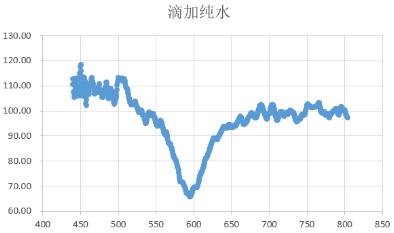
\includegraphics[width=180pt]{images/3_1.png}
%     \end{minipage}
%     \hspace{10pt}%
%     \begin{minipage}[htpb]{180pt}
%       \centering
%       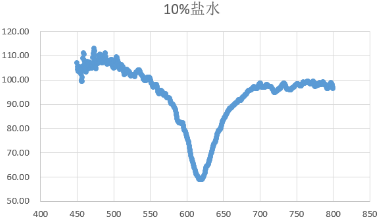
\includegraphics[width=180pt]{images/3_2.png}
%     \end{minipage}
%     \end{figure}
% \end{frame}
% \begin{frame}{各液体光谱图像}
%   \begin{figure}[htbp]
%     \centering
%     \begin{minipage}[htbp]{180pt}
%       \centering
%       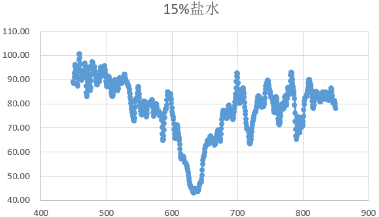
\includegraphics[width=180pt]{images/3_3.png}
%     \end{minipage}
%     \hspace{10pt}%
%     \begin{minipage}[htpb]{180pt}
%       \centering
%       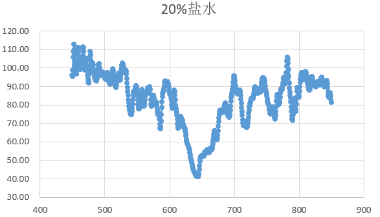
\includegraphics[width=180pt]{images/3_4.png}
%     \end{minipage}
%     \end{figure}
% \end{frame}
% \begin{frame}{各液体光谱图像}
%   \begin{figure}[htbp]
%     \centering
%     \begin{minipage}[htbp]{180pt}
%       \centering
%       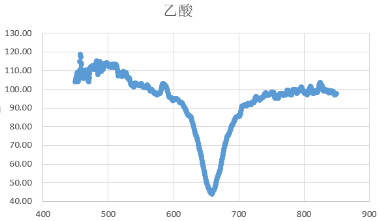
\includegraphics[width=180pt]{images/3_5.png}
%     \end{minipage}
%     \hspace{10pt}%
%     \begin{minipage}[htpb]{180pt}
%       \centering
%       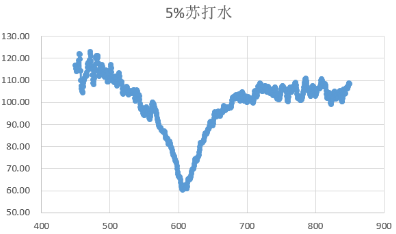
\includegraphics[width=180pt]{images/3_6.png}
%     \end{minipage}
%     \end{figure}
% \end{frame}

% \begin{frame}{各液体光谱图像}
%   \begin{figure}
%     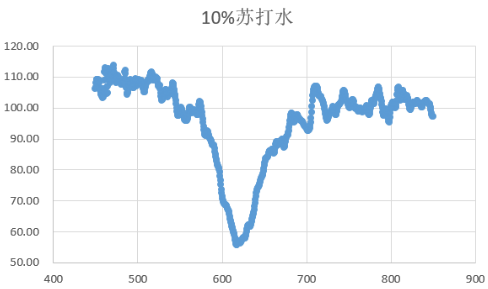
\includegraphics[width=180pt]{images/3_7.png}
%   \end{figure} 
%   将数据总结,表格如下:
%   \begin{table}
%     \scriptsize
%   \begin{tabular}{rlllllll}
%     \toprule
%     液体& 纯水& 5\%苏打& 10\%苏打& 10\%盐水& 15\%盐水& 20\%盐水& 乙酸\\
%     \midrule
%     折射率& 1.335& 1.3405& 1.3460& 1.3501& 1.3571& 1.3683& 1.375\\
%     共振波长& 595& 606& 617& 620& 635& 644& 659\\
%     共振深度& 34.2& 45& 46.2& 38.1& 40& 49.9& 55\\
%     共振宽度& 45& 51& 52& 45& 50& 53& 53\\
%     \bottomrule
%     \end{tabular}
%   \end{table}
% \end{frame}

% \begin{frame}{实验数据}

%   绘制图像为:
%   \begin{figure}
%     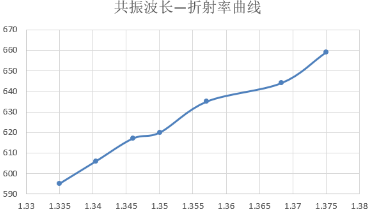
\includegraphics[width=180pt]{images/2_8.png}
%   \end{figure}
%   共振波长呈单调递增趋势,与理论仿真是相符合的。
% \end{frame}

% \begin{frame}
%   \frametitle{实验图像}
%   \begin{figure}
%     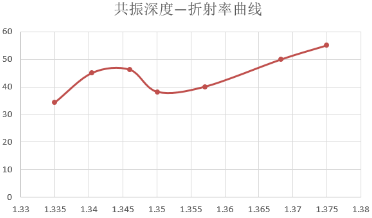
\includegraphics[width=180pt]{images/2_9.png}
%   \end{figure}
%   \begin{figure}
%     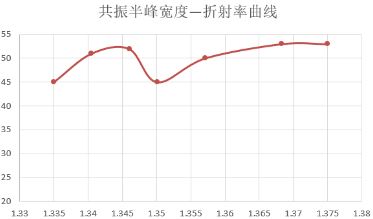
\includegraphics[width=180pt]{images/2_10.png}
%   \end{figure}
% \end{frame}

% \begin{frame}
%   \frametitle{实验分析}
%   \begin{itemize}
%     \item 共振深度和共振半峰宽度理论上也应该是单调递增关系,但是我们测得的数据却有两个不正常的点,是5\%的苏打水和10\%的苏打水
%     \item 之所这两个点偏离了曲线,是因为我们在测量完盐水和乙酸后,去测苏打水时,觉得金片受溶液污染较严重,于是重新拿下来清洗后再放上去重新调光路
%     \item 在这一步我们犯的错误就是改变了参考光,理论上在这个实验中,为了控制变量,我们必须保证测所有液体时参考光是不变的,一旦改变参考光,对于实验结果会有很大的影响
%   \end{itemize}
% \end{frame}

% \section{总结反思}

% \begin{frame}
%   \frametitle{遇到的问题}
%   \begin{itemize}
%     \item 调整光路时,始终测不到光谱值,尽管在接收处已经看到光斑,还是看不到光谱。在老师的指点下,我们知道我们首先需要调整接收机与光线同轴,需要用擦镜纸在接收处观察棱镜反射过来的光斑和光纤端面反射过来的光斑,将二者调整到重合与接收面中心处。然后,我们可以先将光纤拆下来,在接收机后用擦镜纸观察是否有光线透射出来,是否在光纤端面中心,调整后再将光纤接上,最后观察到光谱之后再进行微调,尽量使得光谱值最大
%     \item 实验中,发现被测液体的滴加数量对实验图像也有较大影响,不知道应控制在多少合适,问过老师后才知道其实只要液体将棱镜的传感区覆盖即可,实验中要求的是将其调整至中心,我们开始忽略了这一点,后来调整后就改进了许多
%   \end{itemize}
% \end{frame}
% \begin{frame}
%   \frametitle{心得收获}
%   \begin{itemize}
%     \item 思考问题、解决问题的能力
%     \item 面对困难问题的心态调整能力
%     \item 合作协助的重要性
%   \end{itemize}
% \end{frame}





% In this slide, some important text will be
% \alert{highlighted} beause it's important.
% Please, don't abuse it.

% \begin{block}{Remark}
% Sample text
% \end{block}

% \begin{alertblock}{Important theorem}
% Sample text in red box
% \end{alertblock}

% \begin{examples}
% Sample text in green box. "Examples" is fixed as block title.
% \end{examples}

%---------------------------------------------------------
%Two columns
% \begin{frame}
% \frametitle{Two-column slide}

% \begin{columns}

% \column{0.5\textwidth}
% This is a text in first column.
% $$E=mc^2$$
% \begin{itemize}
% \item First item
% \item Second item
% \end{itemize}

% \column{0.5\textwidth}
% This text will be in the second column
% and on a second tought this is a nice looking
% layout in some cases.
% \end{columns}
% \end{frame}